%!TEX root=main.tex
\section{FPGA 内部并行化}
\label{clicknp:sec:optimization}

充分利用FPGA内部的并行性对性能至关重要。
\name 充分挖掘元件间和元件内的FPGA并行性。

\subsection{元件间并行化}
\name 的模块化体系结构使得在不同元件之间利用并行性变得很自然。
\name 工具链将每个元件映射到FPGA中的硬件模块。
这些硬件模块通过 FIFO 缓冲区互连,可以完全并行工作。 
因此,可以将 \name 配置中的每个元件视为具有自定义逻辑的微小独立核心。
数据包沿着\textit {处理管道}从一个元件流向另一个元件。
这种类型的并行性称为\textit {流水线并行}。
此外,如果单个处理流水线没有足够的处理能力,可以在FPGA中复制多个这样的流水线,并使用负载平衡元件将数据划分到这些流水线中,即利用\textit{数据并行}。
对于网络流量,存在数据并行性(在数据包级或流级别)和流水线并行性,可用于加速处理。
\name 非常灵活,可以轻松配置两种类型的并行,如图 \ref{clicknp:fig:element-para}。

\begin{figure}
\centering
\begin{tabular}{c}
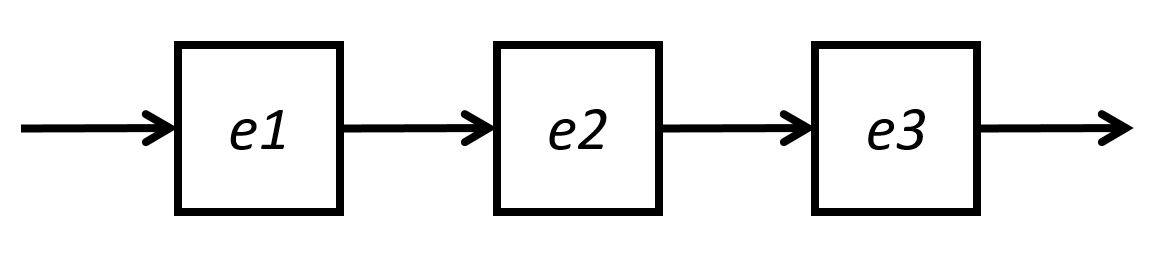
\includegraphics[width=0.56\textwidth]{pipeline.jpg}\\
(a)\\
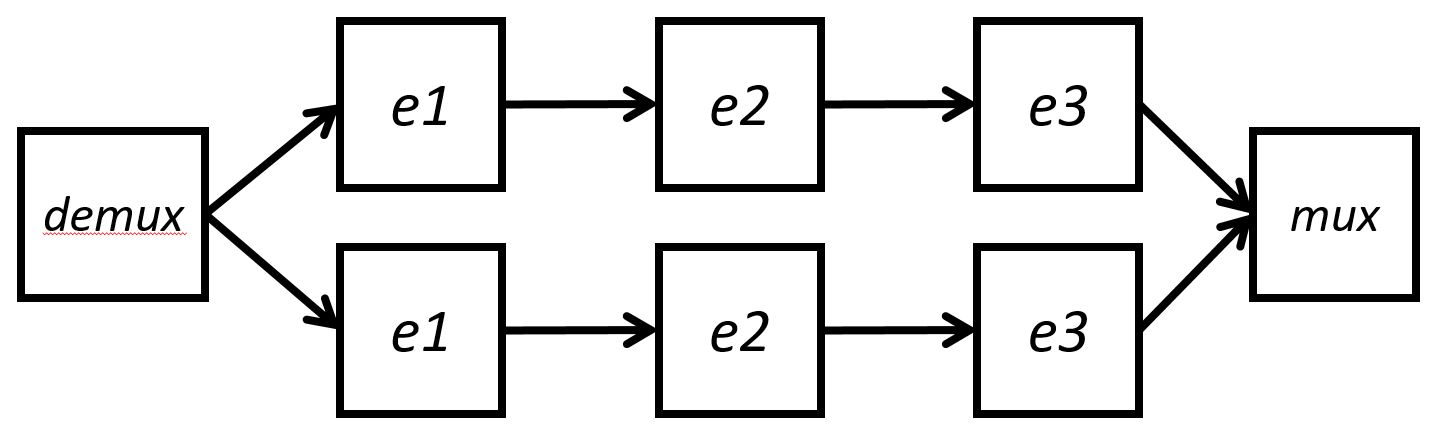
\includegraphics[width=0.7\textwidth]{data.jpg}\\
(b)\\
\end{tabular}
\caption{(a) 元件间并行。 (b) 元件内并行。}
\label{clicknp:fig:element-para}
\end{figure}

开发者可以手工指定元件间并行的次数(即某个元件重复的次数),也可以指定整个网络功能流水线或某个元件的吞吐量或面积目标,由 \name 工具链自动计算各元件的并行次数。\name 根据高层次综合工具输出的依赖分析报告得到平均每时钟周期最多从输入管道读取的数据量,并根据 FPGA 综合后的时钟频率估计元件的吞吐量 \footnote{假定元件内部无阻塞,即每次迭代都能从输入管道中读入数据。如果元件不能做到,开发者可以指定每次读入数据所需的平均迭代次数。};根据 FPGA 的综合结果得到面积。\name 工具链自动平衡各个元件的复制次数,使得流水线中各个元件的处理吞吐量大致平衡。

\subsection{元件内并行}
\label{clicknp:subsec:paral_in_elem}

与在内存中以有限并行性执行指令的CPU不同,FPGA将操作合成为硬件逻辑,因此可以消除指令加载开销。
如果数据在一个处理函数中需要多个相关操作,则高层次综合工具将以同步方式将这些操作调度到管道阶段。
在每个时钟,一个阶段的结果移动到下一个阶段,同时,一个新的数据被输入到这个阶段,如图 \ref{clicknp:fig:dependency}(a)所示。
这样,处理函数可以在每个时钟周期处理数据并实现最大吞吐量。
但是,实际上,流水线处理可能会在两种情况下效率降低:(1)操作中存在\textit {内存依赖}; (2)有\textit {不平衡} 的流水线阶段。
以下两个小节将详细讨论这两个问题,并提出解决方案。
%Finally, in \S~\ref{clicknp:subsubsec:pipeline-control}, we discuss how to explicitly
%control the pipelining to get better clock frequency in \name.



\subsubsection{减少内存依赖}


如果两个操作访问相同的内存位置,并且其中至少有一个是 \textit {写操作},这两个操作被称为相互依赖 \cite {dependence}。
因为每个内存访问都有一个周期延迟,并且程序的语义正确性很大程度上取决于操作的顺序,具有 \textit {内存依赖}的操作无法同时处理。
如图 \ref {clicknp:fig:dependency}(b),\textbf {S1}和 \textbf {S2}相互依赖:\textbf {S2}必须延迟到\textbf {S1}结束 ,只有在\textbf {S2}完成后,\textbf {S1}才能对新的输入数据进行操作。
因此,该函数将需要两个周期来处理一个数据。
对于某些数据包处理算法,内存依赖性可能相当复杂,但是由于 \name 的模块化体系结构,大多数元件只执行简单的任务,而\textit {读写操作}之间的内存依赖关系是最常见的情况,如图 \ref{clicknp:fig:dependency}(b)所示。

消除此内存依赖性的一种方法是仅将数据存储在寄存器中。
由于寄存器足够快,可以在一个周期内执行读取,计算和写回,只要计算过程可在一个时钟周期内完成,根本就不存在\textit {读写}依赖。
与CPU相比,FPGA的寄存器数量要大得多,如Altera Stratix V有697Kbit的寄存器,因此可以使用寄存器尽可能减少内存依赖性。
当变量是标量,或者变量是数组但所有访问的偏移量均为常量且数组大小不超过阈值时,\name 编译器将该变量在寄存器中实现。
程序员可以使用 ``register'' 或 ``local / global'' 关键字来明确地指示编译器放置一个变量(也可以是一个数组)在寄存器,BRAM或板载DDR内存。

对于较大的数据,它们必须存储在BRAM或DDR内存中。
元件内声明的变量默认存储在 BRAM 中。
幸运的是,仍然可以使用一种名为\textit {延迟写入}的技术缓解图 \ref {clicknp:fig:dependency}(b)中\textit {读写操作}导致的内存依赖 \footnote{图 \ref {clicknp:fig:dependency}(b)中写操作的结果可能在下一次循环迭代中被读操作使用。展开相邻的两次循环迭代后,读后写和写后读本质上是同种依赖。}。
延迟写入的核心思想是通过增加临时存储来缓解内存依赖。
延迟写入将待写入的新数据缓冲在寄存器中,直到下一次读操作 \footnote{\textit{延迟写入}得名于变换后的代码模式,在物理上写入到内存的操作并没有被延迟。延迟写入技术生成的硬件逻辑是流水线处理器设计中常用的寄存器转发(register forwarding)模式。}。
如果下一次读取访问相同的位置,它将从缓冲寄存器中直接读取值。
这样,读操作和写操作可以并行执行,因为读写操作一定访问不同的内存位置。
\footnote{FPGA中的大多数BRAM都有两个端口,一个用于读操作,一个用于写操作,即每个时钟周期可以执行一次随机读和一次随机写,读写操作分别有一个时钟周期的延迟。}
图 \ref {clicknp:fig:dependency}(c)显示了延迟写入的代码片段。
由于代码中不再存在内存依赖性,元件可以每个周期处理一个数据,实现完全流水线化。
默认情况下,\name 编译器会对存在读写依赖的数组自动应用 \textit {延迟写入},生成类似图 \ref {clicknp:fig:dependency}(b)的代码。
如果存在读写依赖的数组有多处读操作,\name{} 将为每处读操作分别生成图 \ref {clicknp:fig:dependency}(c)中 P1 所示的代码。
如果数组有多处写操作,且这些写操作位于互斥的分支条件中,\name{} 将生成中间寄存器变量,转化成仅有一处写操作的情形。
如果数组有多处不互斥的写操作,目前 \name{} 不能自动生成延迟写入。
\footnote{理论上可以如下实现:如果有 $N$ 处写操作,可以用 $N$ 个寄存器保存这些写入的值,并在读取时比较所有 $N$ 个寄存器。如果读写操作之间互相穿插,而生成的内存读写指令集中于一处,还需要增加寄存器以保存中间状态。}


\begin{figure}
\lstset{style=numbers}

\lstset{ emph={%
 element, init, state, handler, signal,include
}, emphstyle={\bfseries .},
morekeywords={get_input_port,read_input_port,from_tor, to_tor, set_output_port, host} 
}

\centering
\begin{tabular}{c}

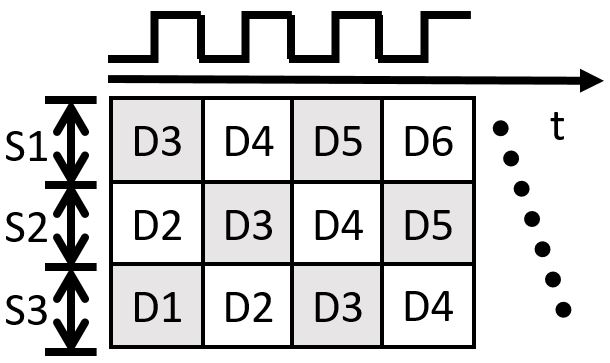
\includegraphics[width=.5\textwidth]{pipeline-w-data.jpg} \\
(a) \vspace{3pt} \\
{
\begin{lstlisting}[escapechar=@]
    r = read_input_port (in);
S1: y = mem[r.x]+1;
S2: mem[r.x] = y;
    set_output_port (out, y);
\end{lstlisting} 
}\\
(b) \vspace{3pt}\\
{
\small
\begin{lstlisting}[escapechar=@]
    r = read_input_port (in);
P1: if ( r.x == buf_addr ) {
       y_temp = buf_val;
    } else {
       y_temp = mem[r.x];
    }
    mem[buf_addr] = buf_val;   
S1: y = y_temp + 1;
S2: buf_addr = r.x;
    buf_val  = y;
    set_output_port (out, y);
\end{lstlisting} 
}\\
(c)
\end{tabular}
\caption{内存依赖的例子。 (a)没有依赖性。 S$n$ 表示流水线的一个阶段,D$n$是一个数据。(b)当状态存储在内存中并需要更新时,会发生内存依赖性。 (c)使用延迟写入解决内存依赖性。}

\label{clicknp:fig:dependency}
\end{figure}

% registers
\egg{
\smalltitle{Use registers.}
Unlike CPU, which executes instructions in memory one by one, FPGA synthesizes 
operations into hardware logic and stores data in registers, and therefore 
can be evaluated in parallel.
For example, Figure~\ref{clicknp:fig:dependency}(a), it may take a CPU two cycles 
to execute \textbf{S1} and \textbf{S2}, while in FPGA, the value of variable 
\textit{y} and \textit{z} can be evaluated in one cycle using 
combinational logic, if we store all variables in registers.
FPGA usually has a large number of registers, \ie, 697Kbit for Altera 
Stratix V, and therefore \name\ aggressively assigns scalar variables 
using registers to increase the parallelism.
}

%\smalltitle{Remove pseudo-dependency.}
使用\textbf {struct}数据结构时会出现一个微妙的问题。
图 \ref {clicknp:fig:memscattering}(a)显示了这样一个例子,其中哈希表用于维护每个流的计数。
\textbf {S2}与\textbf {S1}间将具有内存依赖关系,尽管它们正在访问\textbf {struct}的不同字段。
原因是几乎所有当前的高层次综合工具都会将\textbf {struct}数据结构视为具有较大位宽的单个数据 -- 等于\textbf {struct}的大小,并且只使用一个仲裁器控制访问。
这种类型的内存依赖性称为\textit {伪依赖}。
在物理上,两个字段\textit {key}和\textit {cnt}可以位于不同的内存位置。
为了解决这个问题,\name 采用了一种名为\textit {内存散射}的技术,它自动将\textbf {struct}数组转换为几个独立的数组,每个数组用于存储\textbf {struct}中的一个字段。每个数组分配不同的BRAM,因此可以并行访问(图 \ref {clicknp:fig:memscattering}(b))。
使用\textit {内存散射}后,\textbf {S1}不再依赖于\textbf {S2},从而消除了伪依赖。
一般地,如果一个数组的所有访问可被划分为若干互不相交的等价类,每个等价类中的访问地址范围互不相交,就可以应用\textit{内存散射},将每个等价类所访问的地址范围转换为一个独立的数组 \footnote{例如图 \ref {clicknp:fig:memscattering} 的例子中,S1 访问除 16 余 0 ~ 7 的地址,S2 访问除 16 余 8 ~ 15 的地址。}。
值得注意的是,内存散射仅适用于FPGA中的元件,如果元件在主机CPU上运行则禁用。

\begin{figure}
\lstset{style=numbers}

\lstset{ emph={%
 element, init, state, handler, signal,include,state\_machine, goto_state
}, emphstyle={\bfseries},
morekeywords={get_input_port,read_input_port,from_tor, to_tor, set_output_port, host, begin, VLAN, IPv4, GRE} 
}
\centering
\small

\begin{tabular}{cc}
\begin{lstlisting}[escapechar=@]
struct hash_entry
{
  ulong key;
  ulong cnt;
} A[100];

.handler {
  ...
  idx = hash (h);
S1: if (A[idx].key==k)
  {
S2: A[idx].cnt ++;
  }
  ...
}
\end{lstlisting} &
\raisebox{-60pt}{
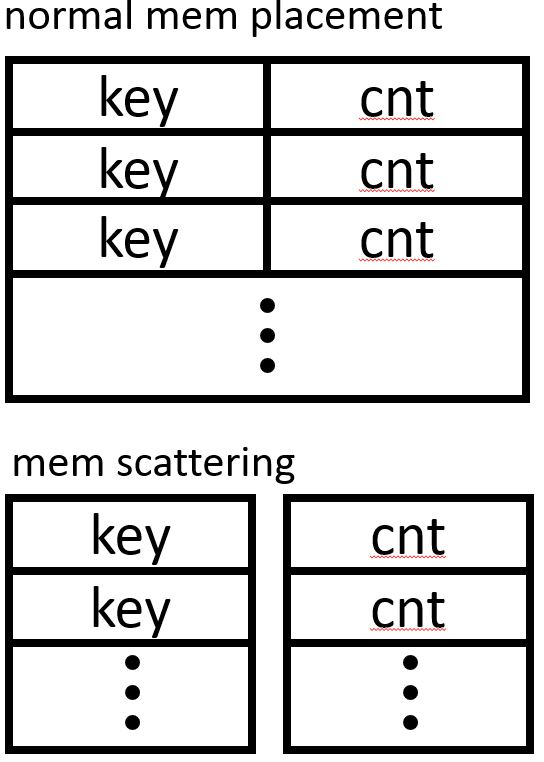
\includegraphics[width=.3\textwidth]{mix.jpg} }\\
(a) & (b)
\end{tabular}

\caption{内存散射。}
\label{clicknp:fig:memscattering}
\end{figure}


当 \textbf{struct} 与 \textbf{union} 共用时,如数据包头有时按字段处理,有时按字节处理,上述内存散射技术不再适用。为了消除数据依赖,\name 采用\textit{数据重排}技术,将 \textbf{union} 中每种类型的数据转换为分立的数组,并根据数据流在数组间同步数据。
一般地,如果一个数组的访问按照程序语句的顺序可被划分为若干个阶段,其中每个阶段的数组访问均符合应用\textit{内存散射}技术的条件,\name 将尝试在阶段间插入数据重排代码,并权衡数据重排的开销与内存散射的收益,选择最优的阶段划分\footnote{例如图 \ref {clicknp:fig:memscattering} 中,如果 A 数组是从输入管道中读入的,则数据读入阶段和 S1 之间需要插入数据重排代码,将 A 数组的内容分别搬移到内存散射后 S1 和 S2 对应的数组。显然,只有当每次读入数据后 S1 和 S2 执行的次数足够多时,数据重排才有收益。}。
数据重排仅适用于 FPGA 上的元件。

上述技术可能无法解决所有内存依赖性。
一些情况下,尽管理论上数据访问可能存在依赖,但程序的输入或计算逻辑隐式保证了不会发生读写冲突。此时程序员可以通过 \texttt{\#pragma ivdep} 来指定某段代码并不存在依赖,高层次综合工具将不再分析这些依赖关系。
在许多情况下,为了确保在FPGA中完全流水线化,程序员需要将代码重写为访问不相交内存区域的多个元件。


\subsubsection{平衡流水级}
理想情况下,一个处理管道中的每个阶段应当具有相同的速度。即,在一个时钟周期处理数据。
但是,如果每个阶段的过程不平衡并且某些阶段需要比其他阶段更多的时钟周期,则这些阶段将限制管道的整个吞吐量。
例如,在图 \ref {clicknp:fig:unbalance}(a)中,\textbf {S1}是一个循环操作。
由于每次迭代需要一个周期(\textbf {S2}),整个循环将需要$N$周期才能完成,从而显着降低了管道吞吐量。
图 \ref {clicknp:fig:unbalance}(b)显示了另一个示例,它为DDR中的全局表(\textit {gmem})实现了一个 BRAM 缓存。
虽然 ``else'' 分支很少命中,但它会在管道中产生一个胖阶段(需要数百个时钟周期)。
我们使用的高层次综合编译器为每个阶段预留最坏情况的时钟周期数量,因此,即使胖阶段很少被用到,也会大大影响整个流水线的处理速度。

\begin{figure}
\lstset{style=numbers}

\lstset{ emph={%
 element, init, state, handler, signal,include,state\_machine, goto_state
}, emphstyle={\bfseries},
morekeywords={get_input_port,read_input_port,from_tor, to_tor, set_output_port, host, begin, VLAN, IPv4, GRE} 
}
\centering

\begin{tabular}{c}
{
\small
\begin{lstlisting}[escapechar=@]
.handler {
   r = read_input_port (in);
   ushort *p = (ushort*) &r.fd.data;
S1: for (i = 0; i<N; i++) {
S2:  sum += p[i];
   }
   set_output_port (out, sum);
}
\end{lstlisting} 
} \\
(a) \vspace{3pt} \\
{
\small 
\begin{lstlisting}[escapechar=@]
.handler {
   r = read_input_port (in);
   idx = hash (r.x);
S1: if ( cache[idx].key == r.x ) {
     o = cache[idx].val;
S2: } else {
     o = gmem[r.x];
     k = cache[idx].key;
     gmem[k] = cache[idx].val;
     cache[idx].key = r.x;
     cache[idx].val = o;
   }
   set_output_port (out, o);
}
\end{lstlisting} 
} \\
(b) \vspace{3pt} 
\end{tabular}

\caption{不平衡的流水级。}
\label{clicknp:fig:unbalance}

\end{figure}


\name 使用两种技术来平衡管道内的各个阶段。首先,尽可能地展开(\textit {unroll})循环。
循环展开可以将循环分解为一系列可并行或流水线执行的小操作。
值得注意的是,展开循环将复制循环体中的操作,从而增加面积成本。
因此,它可能仅适用于具有简单循环体和少量迭代的循环。
在网络功能中,这种小循环是相当常见的,例如计算校验和,对数据包有效负载进行移位,或者迭代枚举各种可能的配置。
\name{} 编译器提供 \textbf {unroll} 指令来展开循环。

虽然许多高层次综合工具支持展开已知迭代次数的循环,但很多现实应用的循环迭代次数是不固定的。
然而,在网络功能中,往往可以确定循环迭代次数的上界,如数据包的最大长度。
由于循环的迭代器常常用来作为数组索引,这种情况下可以根据数组的大小确定迭代器的上下界 \footnote{\name{} 不支持动态内存分配,因此数组的大小都是编译时可以静态确定的。}。
另有一些循环的迭代器上界是常量或其他循环迭代器组成的简单表达式,这种情况下可以计算上界表达式的最大值。
对于编译器不能自动确定循环迭代次数的情况和没有显式迭代器的 \texttt{while} 循环,\name 允许程序员通过 \texttt{pragma} 指定循环次数的上界。
循环次数上界确定后,\name 将循环体用表示循环条件的 \texttt{if} 语句包裹,替换循环体中的 \texttt{continue} 和 \texttt{break} 语句,然后复制多份。

对图 \ref {clicknp:fig:unbalance}(a)所示的计算,循环展开后还需要解决内存依赖,因为变量 \texttt{sum} 被多次写入和读取。\name 在循环展开后,对标量变量展开为\emph{静态单赋值}(static single assignment)形式,使得每个变量仅被赋值一次,即可消除这种内存依赖。本质上,静态单赋值与延迟写入都是用增加内存空间的方式提高并行性。



第二种技术是,如果元件同时具有快速和慢速操作,可以尝试将单个元件中的每种类型的操作分开。
例如,在缓存元件的实现中,如图 \ref {clicknp:fig:unbalance}(b)所示,较慢的 ``else'' 分支被移动到另一个元件中,使得快速路径和慢速路径异步运行。
如果缓存不命中率很低,则整个元件的处理速度由快速路径决定。
如图 \ref{clicknp:fig:async},\name 编译器提供 ``\texttt{async}'' 原语,用户可以在 \texttt{handler} 中插入 \texttt{async \{ \}} 包裹的代码块,其中的代码将被编译成一个新元件,通过管道与原来的元件相连。原来的元件将异步元件中所用到的变量序列化并发送给异步元件,然后等待异步元件结束。异步元件执行完毕后,将原来元件仍将用到的写入变量发送回原来元件。



\begin{figure}[htbp]
	\small
	\lstset{ emph={%
			element, init, state, handler, signal,include,state\_machine, goto_state, async
		}, emphstyle={\bfseries},
		morekeywords={get_input_port,read_input_port,from_tor, to_tor, set_output_port, host, begin, VLAN, IPv4, GRE} 
	}
	\centering
	\begin{tabular}{c}
\begin{lstlisting}
.handler {
  r = read_input_port (in);
  idx = hash (r.x);
  if (cache[idx].key == r.x) {
    o = cache[idx].val;
  } else {
    k = cache[idx].key;
    v = cache[idx].val;
    .async {
      o = gmem[r.x];
      gmem[k] = v;
    }
    cache[idx].key = r.x;
    cache[idx].val = o;
  }
  set_output_port (out, o);
}
\end{lstlisting}
	\end{tabular}
	\caption{Async 原语示例。}
	\label{clicknp:fig:async}
\end{figure}


\iffalse
\begin{figure}
	
	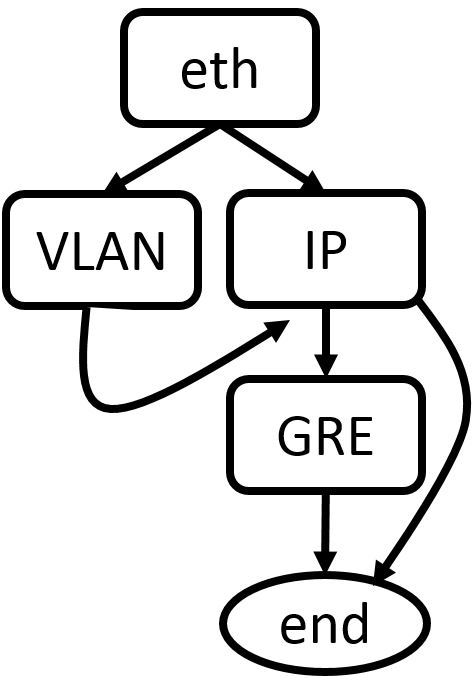
\includegraphics[width=.15\textwidth]{fsm1.jpg} \\
	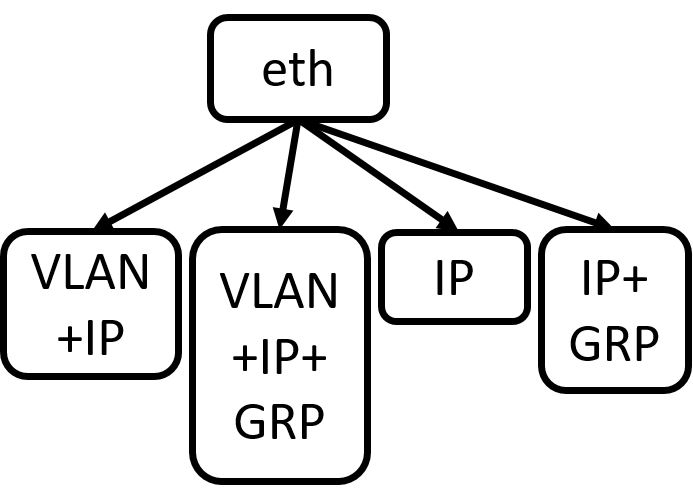
\includegraphics[width=.2\textwidth]{fsm2.jpg} \\
	
	\caption{FSM expansion. }
	\label{clicknp:fig:fsm-expansion}
\end{figure}

\smalltitle{Expand code.} \name\ provides several tools to help programmers to expand code, trading off FPGA area for speed.
One common code expansion is to unroll loops. Additionally, \name\ provides \textit{.repeat} directive to expand code according to
a template.
Finally, \name\ can also help to expand a \textit{finite state machine} (FSM).
Figure~\ref{clicknp:fig:memscattering}(c) shows such an example in packet header parser.
The \textbf{.state\_machine} directive has two functions. First, it provides programmers a declarative way to write a FSM by defining
states and their transitions (using \textbf{.goto\_state}).
Second, it also expends the FSM to get more parallelism. 
For example, Figure~\ref{clicknp:fig:memscattering}(d) shows the parsing tree that is described according to the code piece in Figure~\ref{clicknp:fig:memscattering}(c).
But \name\ compiler can automatically expends the FSM to an equivalent, but much flattened FSM, as shown in Figure~\ref{clicknp:fig:memscattering}(e). Now every header can be parsed in one cycle -- all parsing paths can be evaluated in parallel, 
instead of up to 4 cycles (Figure~\ref{clicknp:fig:memscattering}(d)).

\fi